% !TEX encoding = UTF-8
% !TEX TS-program = pdflatex
% !TEX root = ../tesi.tex

%**************************************************************
\chapter{L'azienda}
\label{cap:azienda}
%**************************************************************
\section{Introduzione}
Wavelop è un’azienda giovane e innovativa, con sede operativa a Treviso e sede legale a Venezia, che si occupa dello \
sviluppo di applicazioni web e \emph{mobile} per \emph{startup} e imprese. L’ambiente è informale e dinamico, con un focus \
alla flessibilità e al lavoro da remoto. L’azienda riesce a soddisfare le richieste dei clienti grazie all’utilizzo della metodologia Agile \emph{Scrum} ed \
alla creazione di \emph{design user-centered}, realizzando \emph{\gls{mock-up}} e prototipi per ottenere i risultati più adatti. \
Vengono, inoltre, utilizzate le migliori tecnologie in base al progetto richiesto.

%**************************************************************
\section{Processi aziendali}

\subsection{Metodologia Agile}
La metodologia Agile è un approccio iterativo al \emph{project management} che consente ai \emph{team} di sviluppo \
di consegnare al cliente il prodotto più rapidamente. In particolare, con lo sviluppo Agile, il \emph{team} si presta a \
lavorare su piccoli incrementi utilizzabili. Ci sono molteplici metodologie che fanno riferimento al \emph{"Agile Manifesto"}, la più diffusa e utilizzata \
dall'azienda, è lo \emph{Scrum}.

\subsection{\emph{Scrum}}
Lo \emph{Scrum} è un \emph{framework} che incoraggia i membri del \emph{team} a lavorare insieme. È basato sul principio dell'apprendimento continuo e sull'adattamento \
a situazioni che cambiano continuamente, mediante ri-prioritizzazione dei processi e brevi cicli di rilascio, chiamati \textbf{\emph{Sprint}}, che permettono al \emph{team} di \
imparare e migliorare. Prima di illustrare come lo \emph{Scrum} venga applicato in Wavelop, è bene introdurre i tre artefatti che sono in continuo aggiornamento durante il progetto:

\begin{itemize}
  \item \textbf{\emph{Product Backlog}}: è la lista dei \emph{tasks} che devono essere svolti e viene mantenuta dal \emph{Product Owner}. La lista contiene \emph{features}, \
  requisiti, miglioramenti e correzioni che fungeranno da \emph{input} allo \emph{Sprint Backlog}. I \emph{tasks} presenti nella lista sono costantemente revisionati, mantenuti \
  e, inoltre, possono subire un cambiamento di priorità; 
  \item \textbf{\emph{Sprint Backlog}}: è la lista dei \emph{tasks} selezionati, durante l'incontro di pianificazione dello \emph{sprint}, dal \emph{team} di sviluppo, per lo \
  svolgimento nello \emph{sprint cycle} corrente. Lo \emph{sprint backlog} può essere flessibile durante lo \emph{sprint}, ma lo \emph{sprint goal} da raggiungere non deve \
  essere compromesso.
  \item \textbf{Incremento} (o \emph{Sprint Goal}): è il prodotto usabile realizzato durante lo \emph{sprint}. Solitamente viene effettuata una dimostrazione al cliente, \
  attraverso una demo, per mostrare il prodotto realizzato durante lo \emph{sprint} e per ottenere \emph{feedbacks} sul lavoro svolto.
\end{itemize}

Prima inizare uno \emph{sprint}, in Wavelop, il \emph{team} si riunisce per definire l'obiettivo dello \emph{sprint} che si andrà a svolgere, inoltre vengono selezionate \
dal \emph{product backlog} le \emph{user stories} che dovranno essere implementate durante lo \emph{sprint}: questa attività prende il nome di \emph{Sprint Planning} e, una volta \
terminata, inizia lo \emph{sprint} vero e proprio. In azienda lo \emph{sprint} dura due settimane, durante le quali il \emph{team} implementa le \emph{user stories} presenti \
nello \emph{sprint backlog}. Durante lo \emph{sprint}, ogni mattina prima di iniziare la giornata lavorativa, viene svolto lo \emph{stand up meeting}: una brave riunione informale \
tra i membri del \emph{team}, durante la quale ci si allinea sul lavoro svolto e si pianifica il lavoro della giornata. Durante l'incontro ogni componente del \emph{team} deve rispondere alle \
seguenti domande: "Cosa ho fatto ieri?", "Cosa farò oggi?", "Ho avuto qualche problema?". Al termine di ogni \emph{sprint}, si svolge una riunione informale tra il \emph{team} e gli \
\emph{\glspl{stakeholder}} per mostrare il lavoro svolto e per ottenere dei \emph{feedbacks} (\emph{Sprint Review}). Successivamente il \emph{team} svolge un'altra riunione per \
discutere su cosa migliorare nel prossimo \emph{sprint} e su cosa ha funzionato nello \emph{sprint} appena concluso (\emph{Sprint Retrospective}). 

\begin{figure}[!ht]
  \begin{center}
    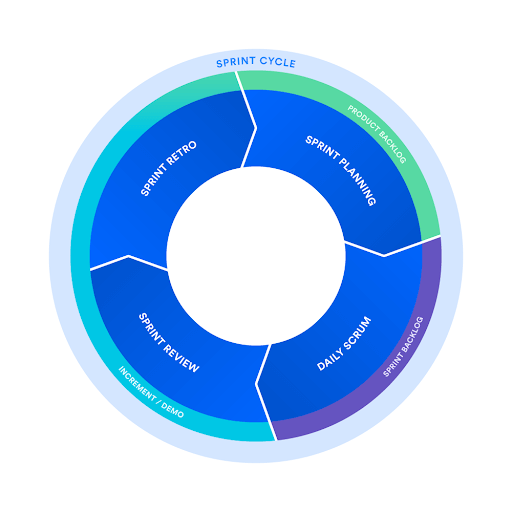
\includegraphics[height=8cm]{sprint-cycle}
    \caption{Ciclo di uno Sprint}
    \textbf{Fonte:} \href{https://www.atlassian.com}{atlassian.com}
  \end{center}
\end{figure}

\subsection{Sviluppo}
Durante la mia permanenza presso l'azienda ho assistito e partecipato al processo di sviluppo, progettando l'architettura del prodotto e implementandola seguendo i principi del \
\emph{Test-Driven Development}. Per realizzare un prodotto di buona qualità è fondamentale mantenere il lavoro ben organizzato, per questo motivo è stato definito un \
\emph{workflow} da seguire per la gestione delle \emph{issues}. \\

Quando una \emph{issue} viene presa in carico, per prima cosa, viene assegnato lo stato \emph{"Doing"}, viene specificato lo sviluppatore a cui essa è assegnata e, se non è già presente, \
viene assegnata la \emph{milestone} dello \emph{sprint} corrente. Prima di iniziarne l'implementazione si devono creare una \emph{merge request} e un \emph{feature branch}, solo dopo \
si può procedere all'implementazione vera e propria. L'implementazione segue il \emph{Test-Driven Development cycle}, ovvero: per prima cosa si scrive un \emph{test}, si esegue il \
\emph{test}, se fallisce si procede a scrivere il codice necessario per farlo passare, successivamente, si eseguono tutti i \emph{test} e solo se tutti hanno successo, se necessario, \
si procede con il \emph{refactoring}. Una volta completata l'implementazione, lo sviluppatore modifica lo stato della \emph{issue} in \emph{"To Review"} e assegna la \
\emph{merge rerquest} a una delle due persone designate dall'azienda. \
Solo in caso di esito positivo si procede con l'aggiunta dei cambiamenti al \emph{branch develop} e la chiusura della \emph{issue} assegnandole lo stato \emph{"Closed"}.

\begin{figure}[!ht]
  \begin{center}
    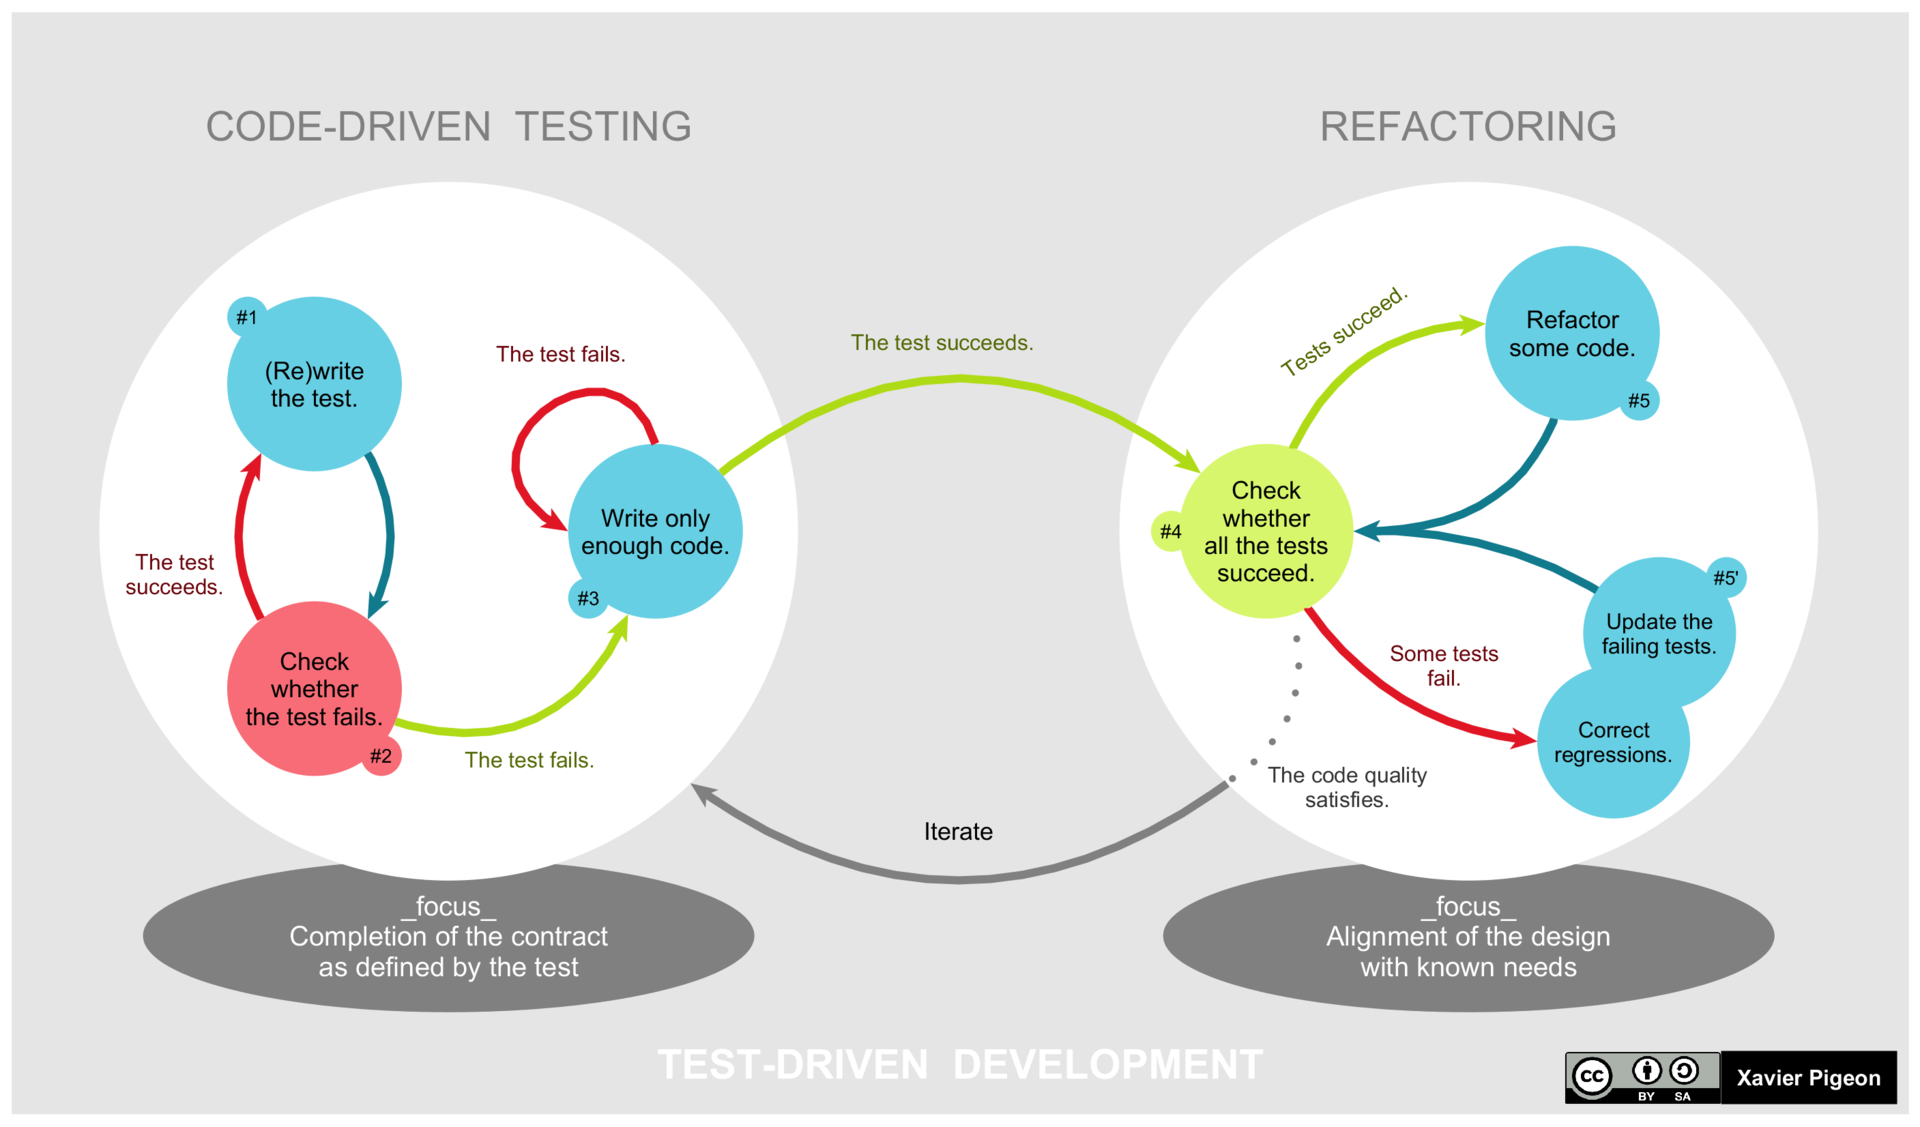
\includegraphics[height=8cm, width=13cm]{tdd-cycle}
    \caption{\emph{Test-Driven Development cycle}}
    \textbf{Fonte:} \href{https://www.wikipedia.org}{wikipedia.org}
  \end{center}
\end{figure}

%**************************************************************
\section{Strumenti a supporto dei processi}

\subsection{\emph{Git} \& \emph{Gitflow Workflow}}
\emph{Git} è un \emph{Distributed Version Control System}, \emph{open-source} e gratuito, progettato per gestire progetti di grandi e piccole dimensioni con efficienza. \
Facendo uso di \emph{way of working} basato su rilasci programmati, l'azienda ha deciso di utilizzare il modello \emph{Gitflow Workflow}. \
Ogni progetto è costituito da cinque tipi di \emph{branch} diversi: \textbf{\emph{main}}, \textbf{\emph{develop}}, \textbf{\emph{release}}, \textbf{\emph{hotfix}} e \
\textbf{\emph{feature}}. I \emph{branches} di base e che saranno sempre presenti nel ciclo di vita del progetto sono:
\begin{itemize}
  \item \emph{main} nel quale si trova lo storico delle versioni rilasciate in produzione dall'azienda;
  \item \emph{develop} nel quale troviamo lo storico completo del progetto. 
\end{itemize}  

I seguenti tipi di \emph{branch}, a differenza dei precedenti, hanno vita limitata: \
\begin{itemize}
  \item i \emph{branch} di tipo \emph{feature} sono adibiti allo sviluppo di nuove funzionalità, al termine del quale viene incorporato nel \emph{branch develop}; 
  \item i \emph{branch} di tipo \emph{release} vengono utilizzati per cominciare un nuovo ciclo di rilascio per una nuova version, al termine del quale viene incorporato nel \
  \emph{branch main}; 
  \item i \emph{branch} di tipo \emph{hotfix} sono adibiti alla correzione di piccoli \emph{bug} in produzione, una volta risolto il problema viene incorporato nel \emph{branch main}.
\end{itemize}

\vspace{10pt}
  \begin{figure}[!ht]
    \begin{center}
      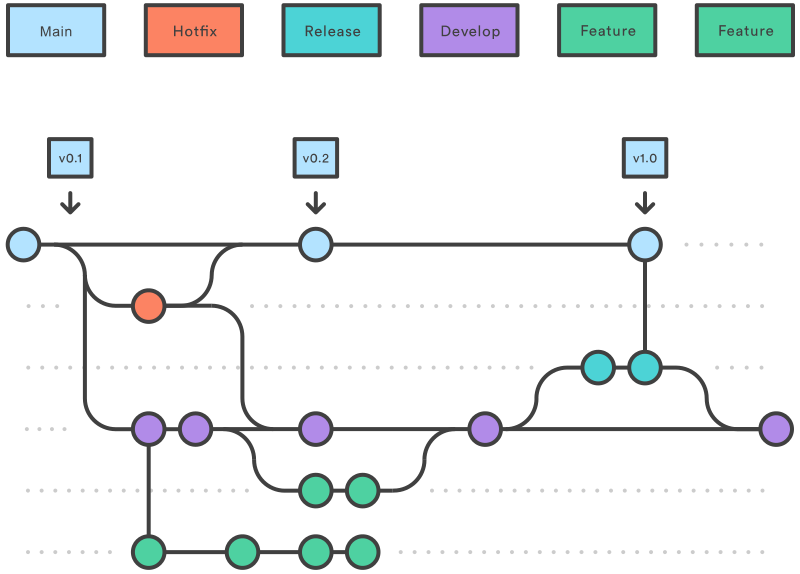
\includegraphics[height=8cm, width=12cm]{gitflow-workflow}
      \caption{Gitflow Workflow}
      \textbf{Fonte:} \href{https://www.atlassian.com}{atlassian.com}
    \end{center}
  \end{figure}
\vspace{10pt} 

\subsection{\emph{GitLab}}
GitLab, a differenza di git, è una piattaforma di \emph{hosting} per \emph{git repositories}; inoltre offre diversi servizi \
per la gestione del progetto, tra i quali:

\begin{itemize}
  \item \emph{Issue Tracking System};
  \item \emph{Project Board};
  \item \emph{Merge Requests}.
\end{itemize}

\subsubsection{\emph{Issue}}
In \emph{GitLab} le \emph{issues} rappresentano i \emph{tasks} da implementare ai fini dell'avanzamento in un progetto. Nel contesto lavorativo di Wavelop, le \emph{issues}, \
sono le \emph{user stories} e sono caratterizzate da: un titolo, una descrizione e uno o più utenti che ce l'hanno in carico; inoltre, viene aggiunta una \
\emph{milestone} (lo \emph{sprint} a cui è asseganta), delle \emph{labels} ai fini di una migliore organizzazione, infine, vengono aggiunti gli \emph{story points} che forniscono \
una stima del tempo che verrà impiegato per implementarla. L'insieme di tutte le \emph{issues} costituesce il \emph{product backlog} mentre le \emph{issues} \
apparteneti ad una determinata \emph{milestone} costituiscono lo \emph{sprint backlog}.
\begin{figure}[!ht]
  \begin{center}
    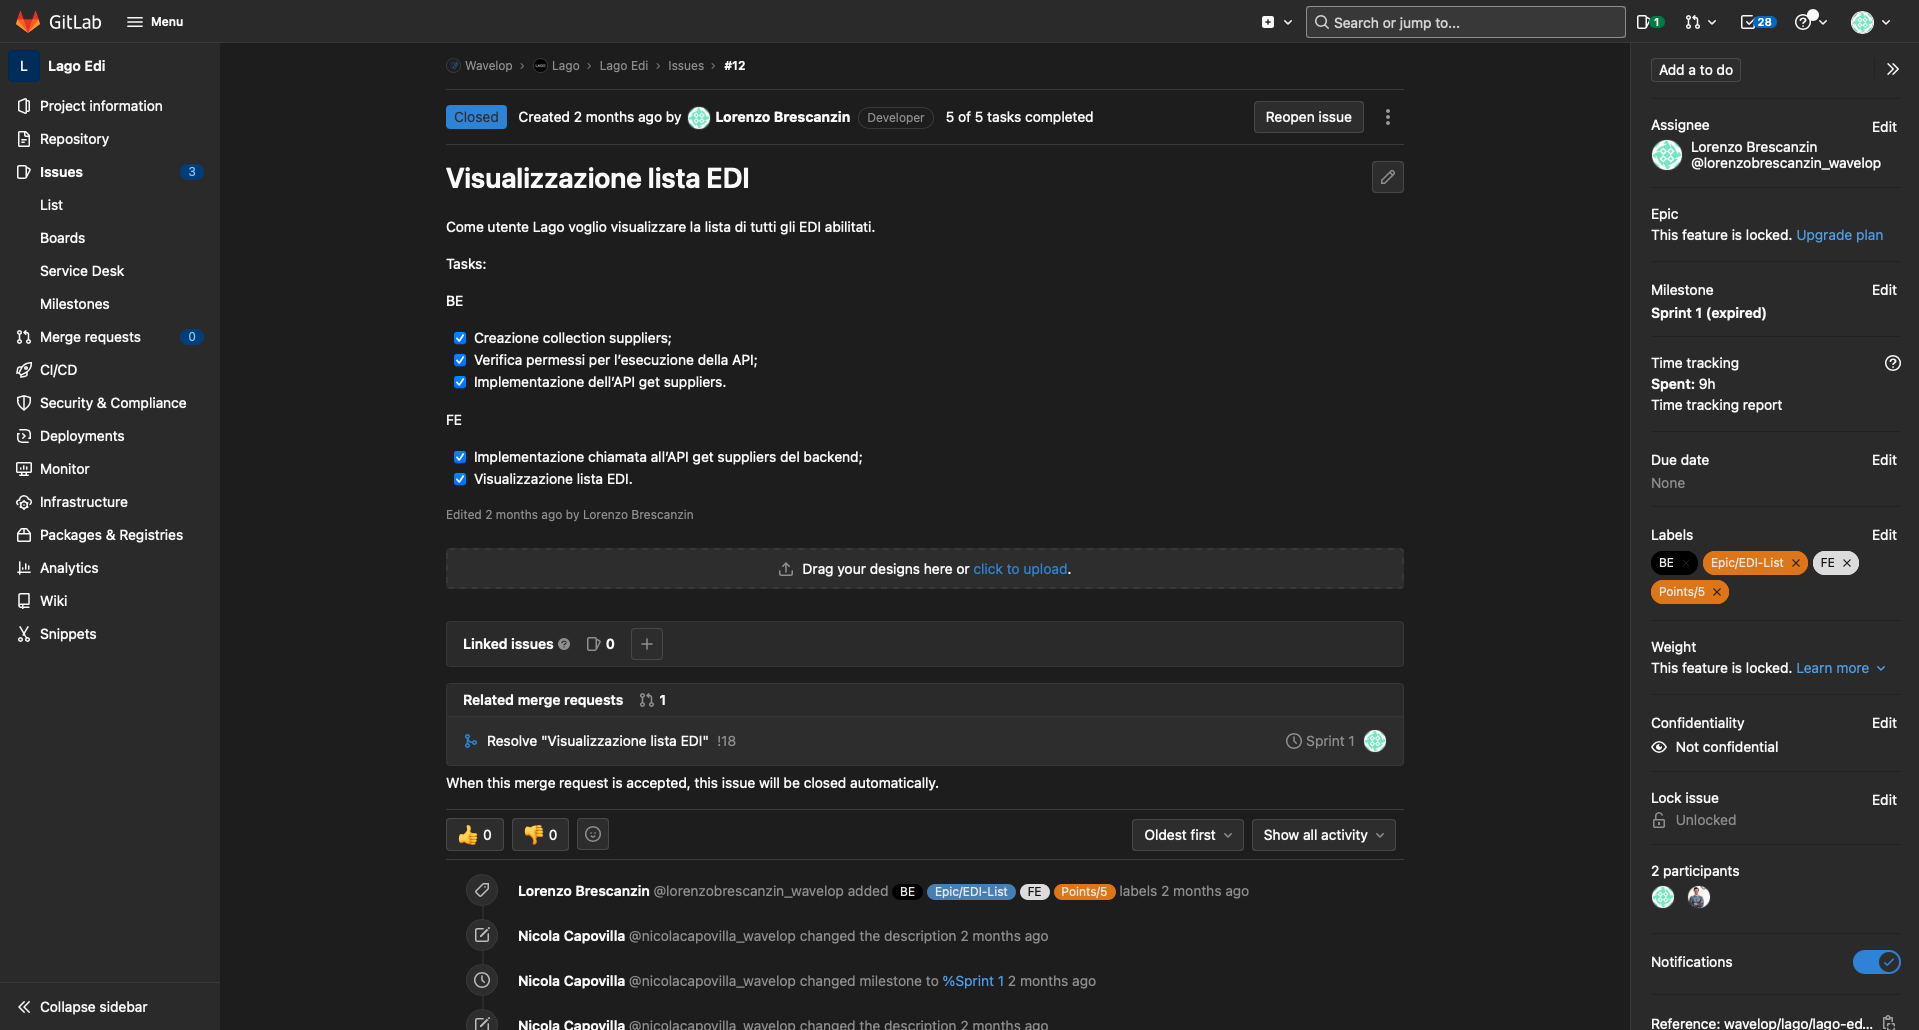
\includegraphics[height=8cm, width=13cm]{issue}
    \caption{Esempio di una \emph{issue}}
  \end{center}
\end{figure}

\subsubsection{\emph{Project Board}}
Una \emph{project board} è un raccoglitore di \emph{issues}, organizzate in colonne, utilizzato per una migliore organizzazione del lavoro e per facilitare \
la verifica dello stato di avanzamento del progetto. In Wavelop la \emph{project board} è costituita da quattro colonne che indicano lo stato in cui si trova una \emph{issue}:

\begin{itemize}
  \item \textbf{\emph{Open}:} la \emph{issue} deve ancora essere presa in carico e quindi deve ancora essere implementata;
  \item \textbf{\emph{Doing}:} la \emph{issue} è stata presa in carico da un componente del \emph{team} ed è in implementazione;
  \item \textbf{\emph{To Review}:} la \emph{issue} è stata implementata ed è pronta per la revisione da parte del \emph{reviewer}. Sulla base dell'esito di questa attività \
  la \emph{issue} viene spostata in \emph{Doing}, nel caso di esito negativo, o in \emph{Closed}, in caso di esito positivo;
  \item \textbf{\emph{Closed}:} la \emph{issue} è stata completata e viene aggiunta al \emph{branch develop}.
\end{itemize}

\begin{figure}[!ht]
  \begin{center}
    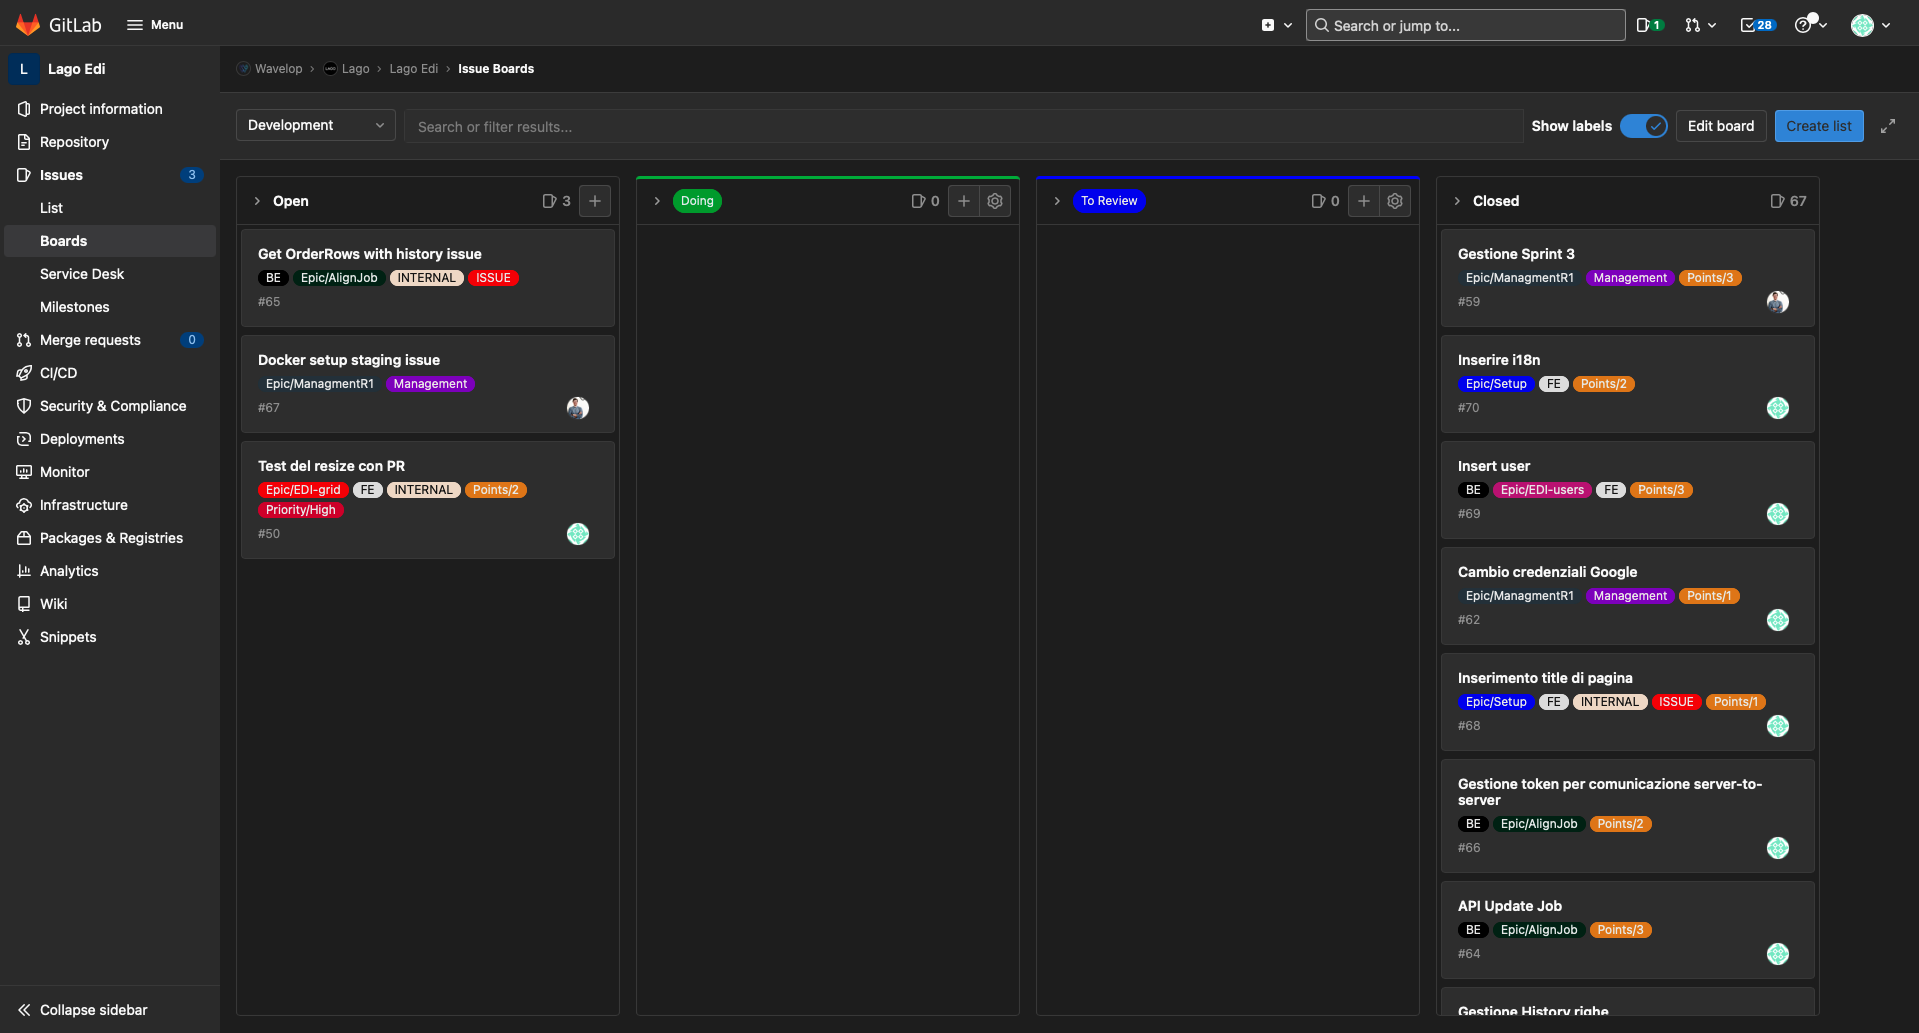
\includegraphics[height=8cm, width=13cm]{project-board}
    \caption{Esempio di \emph{project board}}
  \end{center}
\end{figure}

\subsubsection{\emph{Merge Requests}}
Le \emph{merge requests} vengono utilizzate per tracciare e revisionare i cambiamenti prima che essi vengano incorporati nei \emph{branch main} o \emph{develop}. All'interno del \
\emph{way of working} di Wavelop, vengono utilizzate anche per discutere di ciò che è stato implementato e di modifiche da apportare. Quando si prende in carico una \emph{issue}, si \
crea una \emph{merge request} e un \emph{feature branch}; una volta che il \emph{reviewer} ha approvato i cambiamenti implementati, il \emph{feature branch} viene unito al contenuto \
del \emph{branch develop} e successivamente eliminato.

\begin{figure}[!ht]
  \begin{center}
    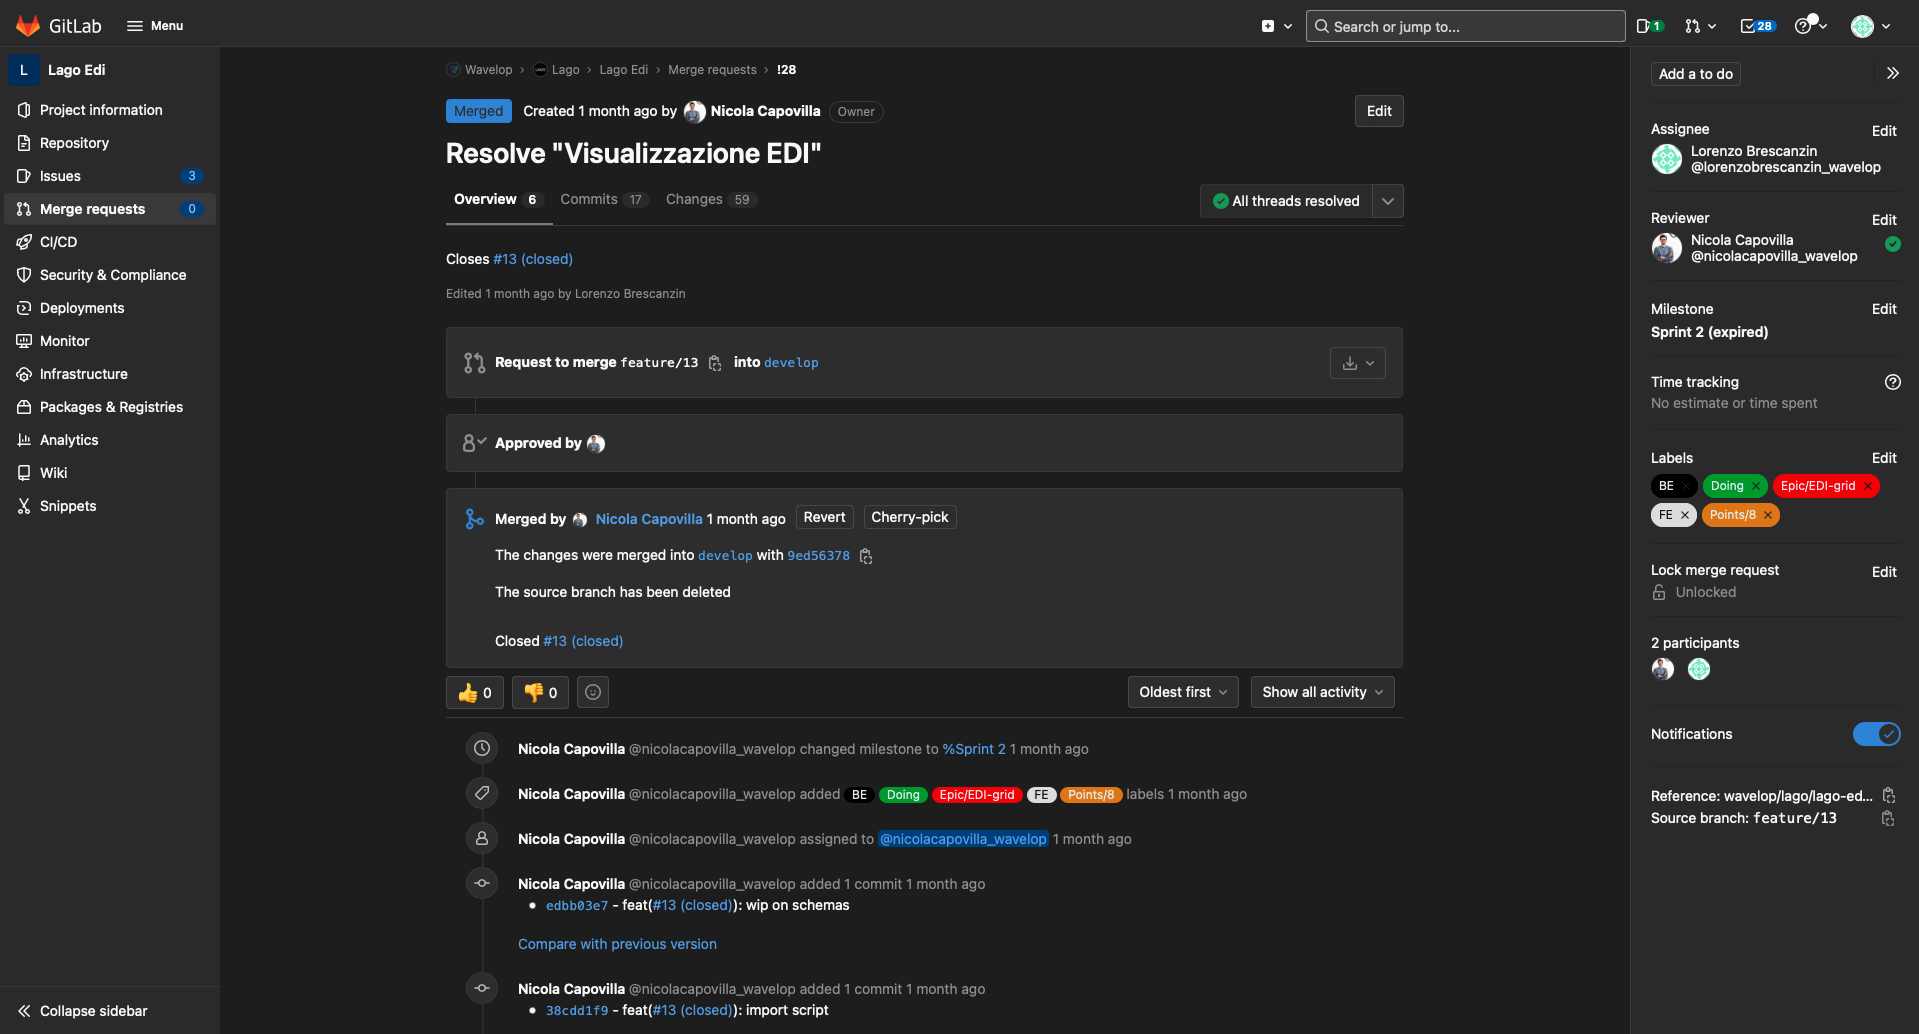
\includegraphics[height=8cm, width=13cm]{merge-request}
    \caption{Esempio di \emph{merge request}}
  \end{center}
\end{figure}

\newpage
\subsection{\emph{Google Workspace}}
\emph{Google Workspace} è un insieme di strumenti di collaborazione e produttività sviluppato da Google. \
I servizi utilizzati maggiormente dall'azienda sono:

\begin{itemize}
  \item \emph{Gmail} per le comunicazioni formali con clienti e \emph{team};
  \item \emph{Calendar} per la gestione degli impegni aziendali;
  \item \emph{Drive} per la memorizzazione di file nel \emph{cloud};
  \item \emph{Meet} per le riunioni formali con i clienti;
  \item \emph{Google Docs Suite} per la redazione della documentazione e per la realizzazione delle presentazioni per i clienti.
\end{itemize}

%**************************************************************
\section{Rapporto con l'innovazione}
L'azienda è in costante aggiornamento sulle nuove tecnologie partecipando ad incontri tecnologici con relatori di spicco: \emph{Google} e \emph{Amazon}, \
per citarne alcuni; in generale, è molto propensa all'innovazione accettando la presa in carico di progetti innovativi che sfruttano \
i moderni \emph{smart speakers}, l'architettura \emph{Serverless} o nell'ambito dell'\acrfull{iot}. Un altro aspetto in cui Wavelop può essere definita innovativa è l'adozione \
del \emph{remote working} sin dagli albori: questa scelta ha permesso ad ogni dipendente di lavorare nelle condizioni in cui performa al meglio, portanto benefici non solo al \
fatturato dell'azienda ma anche alla persona stessa. Grazie all'esperienza maturata nel lavoro da remoto, l'azienda è riuscita a non subire direttamente degli effetti negativi \
della pandemia. Un altro aspetto importante è la costante ricerca di giovani da formare con il \emph{focus} sull'innovazione garantendo così un futuro alla visione aziendale.